\documentclass[11pt]{article}
\usepackage{icmlko}
\begin{document}

\title{위약을 돌리기 전에 결과를 안다 --- 겹침 비율이 잔량을 맞힌다}
\author{월드모델 실험실}
\date{노트 390 · 2026년 8월 1일}
\maketitle

\begin{abstract}
노트 389가 조항 ⑤를 만들었다 --- \emph{학습 행을 더하는 변경은 위약(새 행의
라벨을 자기들끼리 섞기)이 이득을 지워야 채택한다.} 만들자마자 소급해야 할
데가 있었다: \textbf{노트 381의 펀딩 학습 확장(320 $\to$ 2,358)이 위약 없이
채택돼 지금 챔피언 안에 있다.}

돌렸다. \textbf{통과한다.}

\begin{center}
\begin{tabular}{lrrrr}
\hline
A(학습 320) 대비 & 판 차 & 부호 & 펀딩 차 & 부호 \\
\hline
B 지금 챔피언 & $+0.0348$ & 12/12 & $+0.2294$ & 12/12 \\
C \textbf{위약} & $+0.0026$ & 9/12 & $\mathbf{+0.0173}$ & 8/12 \\
\hline
\end{tabular}
\end{center}

위약이 남기는 것이 판에서 7.5\% · 펀딩에서 7.5\% 다. 노트 381의 채택은
정보 때문이었다.

\textbf{그런데 소급하다가 더 쓸모 있는 것이 나왔다.} 이제 조항 ⑤를 적용한
사례가 셋이고, \emph{새 행 중 기존 학습 범위 밖 비율}과 \emph{위약이 남기는
이득 비율}이 거의 같다:

\begin{center}
\begin{tabular}{lrrl}
\hline
변경 & 기존 범위 밖 & 위약 잔량 & 판정 \\
\hline
웹툰 E1 (노트 388) & 10\% & $-8$\% & 채택 \\
펀딩 (노트 381) & 16\% & 7.5\% & 채택 유지 \\
만화 (노트 389) & \textbf{100\%} & \textbf{91\%} & 기각 \\
\hline
\end{tabular}
\end{center}

\textbf{그러면 위약을 돌리기 전에 알 수 있다} --- 새 행의 라벨이 기존 학습
범위 밖에 얼마나 있는지만 세면 된다. 요청 하나도 안 쓰는 계산이고, 팔을
하나 더 적합시키는 값을 아낀다. \textbf{다만 점이 셋이라 법칙이 아니라
검사해야 할 관측으로 적는다} --- 노트 386이 네 점에 곡선을 그리지 말라고
비싸게 가르쳤다.
\end{abstract}

\section{소급 --- 챔피언 안을 먼저 본다}

조항 ⑤를 만든 노트가 그 조항을 안 거친 것을 챔피언에 두고 있으면 앞뒤가
안 맞는다. 학습 행을 더해 채택된 변경이 지금 챔피언에 둘 있다.

\begin{itemize}
\item \textbf{노트 387 웹툰 835편} --- 위약을 그때 돌렸다. 통과했다
($+0.0305 \to -0.0024$).
\item \textbf{노트 381 펀딩 2,038편} --- \textbf{안 돌렸다.} 판 $+0.0322$ ·
12/12 로 채택했고, 그것이 이번 사이클에서 제일 큰 이득이었다.
\end{itemize}

펀딩 쪽을 돌렸다. A는 노트 381 이전(학습 320), B는 지금 챔피언(학습
2,358), C는 B에서 \emph{더한 2,038행의 라벨만} 자기들끼리 섞은 것이다.
유보 529행은 세 팔이 같다.

\textbf{B $+0.0348$(12/12) 대 C $+0.0026$(9/12).} 위약이 이득의 92.5\%를
지운다. \textbf{노트 381은 유지한다.}

(A 대비 차가 노트 381이 보고한 $+0.0322$ 가 아니라 $+0.0348$ 인 것은 그
사이에 웹툰 835편이 들어와 판이 달라졌기 때문이다 --- 노트 371대로 같은
실험 안에서만 견주므로 두 수를 나란히 놓지 않는다.)

\begin{figure}[t]
\centering
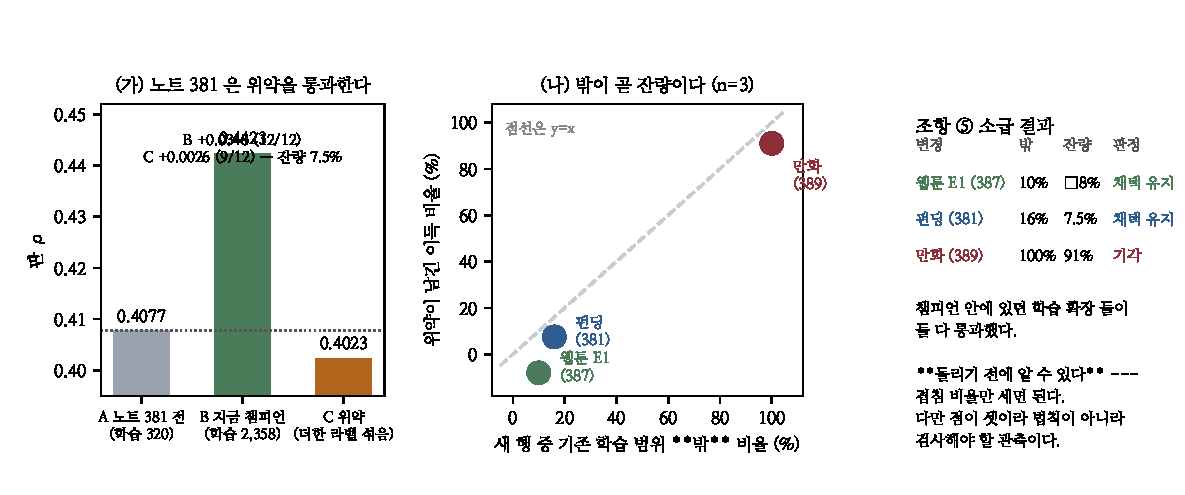
\includegraphics[width=\linewidth]{figs/fig390.pdf}
\caption{\textbf{(가)} 노트 381의 세 팔. 위약(주황)이 A 아래로 떨어진다.
\textbf{(나)} 세 사례에서 ``기존 범위 밖 비율''과 ``위약 잔량''이 $y=x$
근처에 놓인다. \textbf{(다)} 조항 ⑤ 소급 결과.}
\label{fig:main}
\end{figure}

\section{겹침 비율이 잔량을 맞힌다}

노트 389가 만화와 웹툰의 차이를 \emph{겹침}으로 설명했다. 여기에 펀딩이
붙으면서 셋이 됐고, 정성적 설명이 정량적 대응으로 보인다.

\begin{center}
\begin{tabular}{lrrrr}
\hline
 & 기존 학습 범위 & 새 행 범위 & 밖 & 위약 잔량 \\
\hline
웹툰 E1 & 410\,--\,794,328 & 90\,--\,794,328 & 10\% & $-8$\% \\
펀딩 & 9\,--\,10,090 & 1\,--\,3,698 & 16\% & 7.5\% \\
만화 & 5,306\,--\,{\small 32만} & 420\,--\,632 & 100\% & 91\% \\
\hline
\end{tabular}
\end{center}

\textbf{읽는 법.} 기존 범위 안에 들어오는 새 행은 모형에게 \emph{그 구간을
더 촘촘히} 보여 준다 --- 라벨을 섞으면 그 정보가 없어지므로 이득도 없어진다.
기존 범위 밖의 새 행은 \emph{그 구간이 존재한다}는 것을 알려 주는데, 그건
라벨을 섞어도 남는다. 그래서 밖의 비율이 곧 위약이 지우지 못하는 몫이 된다.

\textbf{펀딩이 재미있는 자리다.} 노트 379가 펀딩 목록의 위 19\%만 갖고
있다고 밝혔으니 새 균일 행이 전부 아래일 것 같은데, 실제로는 84\%가 기존
범위 \emph{안}이다. 기존 320행이 상위 구역에서 뽑혔어도 그 안에 후원자
9명짜리부터 만 명짜리까지 있었기 때문이다 --- \textbf{구역 편향은 범위를
자르는 게 아니라 밀도를 비트는 것}이고, 그래서 고치면 정보가 는다.
만화의 경우는 범위 자체가 잘려 있었고, 그 아래를 통째로 붙이면 밀도가
아니라 눈금이 바뀐다.

\section{그래서 절차가 하나 짧아진다}

조항 ⑤는 팔을 하나 더 적합시키라는 요구라 비싸다(이번 관문들에서 12뽑기
$\times$ 팔 하나 $=$ 적합 12회). \textbf{그 앞에 요청 없는 계산을 둔다:}

\begin{enumerate}
\item 새 학습 행의 라벨이 기존 학습 라벨 범위 \textbf{밖}에 몇 \% 인지 센다.
\item 그 값이 크면(지금 근거로는 절반 이상) 위약이 이득을 못 지울 것으로
보고 \textbf{관문을 돌리기 전에} 설계를 고친다 --- 겹치는 구간을 같이
모으거나, 밖에 있는 것을 뺀다.
\item 작으면 관문 $+$ 위약을 정상대로 돌린다.
\end{enumerate}

\textbf{점이 셋이다.} 10/$-8$ · 16/7.5 · 100/91 이 $y=x$ 에 가깝게 놓이지만
가운데가 비어 있다(16\%와 100\% 사이). 30\,--\,70\% 짜리 사례가 나오면
그때 이 대응이 진짜인지 안다. \textbf{그전까지는 관문을 건너뛰는 데 쓰지
않고 설계를 고치는 데만 쓴다} --- 노트 386이 네 점으로 곡선을 그리려다
배운 것이다.

\section{남은 것}

\begin{center}
\begin{tabular}{lll}
\hline
항목 & 왜 값이 큰가 & 어떻게 \\
\hline
가운데 점 & 밖 30\,--\,70\% 사례가 없다 & 만화 633\,--\,5,306 구간을 모으면 그쯤 된다 \\
애니 아카이브 & 무게 606 · 덮음 22\% & 수집 중 · 받으면 밖 비율부터 센다 \\
조항 ⑤ 자동화 & 손으로 세면 빠뜨린다 & 관문 스크립트에 밖 비율을 찍는다 \\
웹툰 나머지 175편 & 덮음 95\% $\to$ 100\% & 수집이 멈췄다 \\
\hline
\end{tabular}
\end{center}

\end{document}
